\documentclass{article} 
\usepackage{cite}
\usepackage[usenames,dvipsnames]{xcolor}
\usepackage{graphicx,bbm,pstricks}
\usepackage{subfigure,pifont}
\usepackage{bm,algorithmic,mdframed,mathtools}
\usepackage{fancyhdr,placeins}
\pagestyle{fancy}
\fancyhead[L]{\slshape \leftmark}
\fancyhead[R]{\slshape PAIS with standard algorithms}
\fancyfoot[C]{\slshape \thepage}
\fancyfoot[R]{\slshape }

\addtolength{\oddsidemargin}{-.4in}
\addtolength{\evensidemargin}{-.4in}
\addtolength{\textwidth}{0.8in}
\addtolength{\topmargin}{-1in}
\addtolength{\textheight}{1.9in}
\fancyhfoffset{0in}
\setlength{\parindent}{0in}
\usepackage{amsmath,amsfonts,epsfig,amsbsy,subfigure}
\newcommand{\RARR}[3]{#1
  \;\displaystyle\mathop{\displaystyle\longrightarrow}^{#3}\; #2}
\newcommand{\RARRlong}[3]{#1
  \;\displaystyle\mathop{-\!\!\!-\!\!\!-\!\!\!-\!\!\!-\!\!\!\!\displaystyle
  \longrightarrow}^{#3}\; #2}
\newcommand{\LARR}[3]{#1
  \;\displaystyle\mathop{\displaystyle\longleftarrow}^{#3}\; #2}
\newcommand{\LRARR}[4]{{\mbox{ \raise 0.4 mm \hbox{$#1$}}} \;
  \mathop{\stackrel{\displaystyle\longrightarrow}\longleftarrow}^{#3}_{#4}
  \; {\mbox{\raise 0.4 mm\hbox{$#2$}}}}
\newcommand{\bX}{{\bf X}}
\newcommand{\vecx}{{\mathbf x}}
\newcommand{\vecy}{{\mathbf y}}
\newcommand{\vecz}{{\mathbf z}}
\newcommand{\vecq}{{\mathbf q}}
\newcommand{\bs}{{\mathbf s}}
\newcommand{\vecr}{{\mathbf r}}
\newcommand{\vecX}{{\mathbf X}}
\newcommand{\vecY}{{\mathbf Y}}
\newcommand{\vecv}{{\mathbf v}}
\newcommand{\tick}{\ding{52}}
\newcommand{\cross}{\ding{54}}
\newcommand{\vecn}{{\mathbf n}}
\newcommand{\vecp}{{\mathbf p}}
\newcommand{\cT}{{\mathcal T}}
\newcommand{\dt}{{\mbox{d}t}}
\newcommand{\dx}{{\mbox{d} \vecx}}
\newcommand{\boldnu}{{\boldsymbol \nu}}
\newcommand{\er}{{\mathbb R}}
\renewcommand{\div}{{\rm div}}
\newcommand{\bnu}{{\bf \nu}}
\newcommand{\divergence}{\mathop{\mbox{div}}}
\renewcommand{\P}{\mathbb{P}}
\newcommand{\FP}{P_{\rm{FP}}}
\newcommand{\ME}{P_{\rm{ME}}}
\newcommand{\MEs}{P_{\rm{ME}_{S}}}
\newcommand{\D}{\mathcal{D}}
\newcommand{\G}{\mathcal{G}}
\newcommand{\N}{\mathcal{N}}
\newcommand{\X}{{\mathbf X}}
\newcommand{\Y}{{\mathbf Y}}
\newcommand{\W}{{\mathbf W}}
\newcommand{\neff}{{n_{\text{eff}}}}
\newcommand{\E}{{\mathbb{E}}}
\newcommand{\I}{{\mathbb{I}}}
\DeclarePairedDelimiter\floor{\lfloor}{\rfloor}
\newcommand{\picturesAB}[6]{
\centerline{
\hskip #4
\raise #3 \hbox{\raise 0.9mm \hbox{(a)}}
\hskip #5
\epsfig{file=#1,height=#3}
\hskip #6
\raise #3 \hbox{\raise 0.9mm \hbox{(b)}}
\hskip #5
\epsfig{file=#2,height=#3}
}}
\newcommand{\picturesCD}[6]{
\centerline{
\hskip #4
\raise #3 \hbox{\raise 0.9mm \hbox{(c)}}
\hskip #5
\epsfig{file=#1,height=#3}
\hskip #6
\raise #3 \hbox{\raise 0.9mm \hbox{(d)}}
\hskip #5
\epsfig{file=#2,height=#3}
}}
\makeatletter
\renewcommand{\@maketitle}{
\newpage
 \null
 \vskip 2em%
 \begin{center}%
  {\LARGE \@title \par}%
 \end{center}%
 \par} \makeatother
\title{PAIS with standard algorithms}

\begin{document}
\thispagestyle{fancy}
\maketitle

\section{Problem 1}
\[
	\mathcal{G}(u) = u, \quad \mu_0 \sim \mathcal{N}(0, 2), \quad \mu_\varepsilon \sim \mathcal{N}(0, 0.1), \quad D = -2.67.
\]
\begin{figure}[h]
\begin{center}
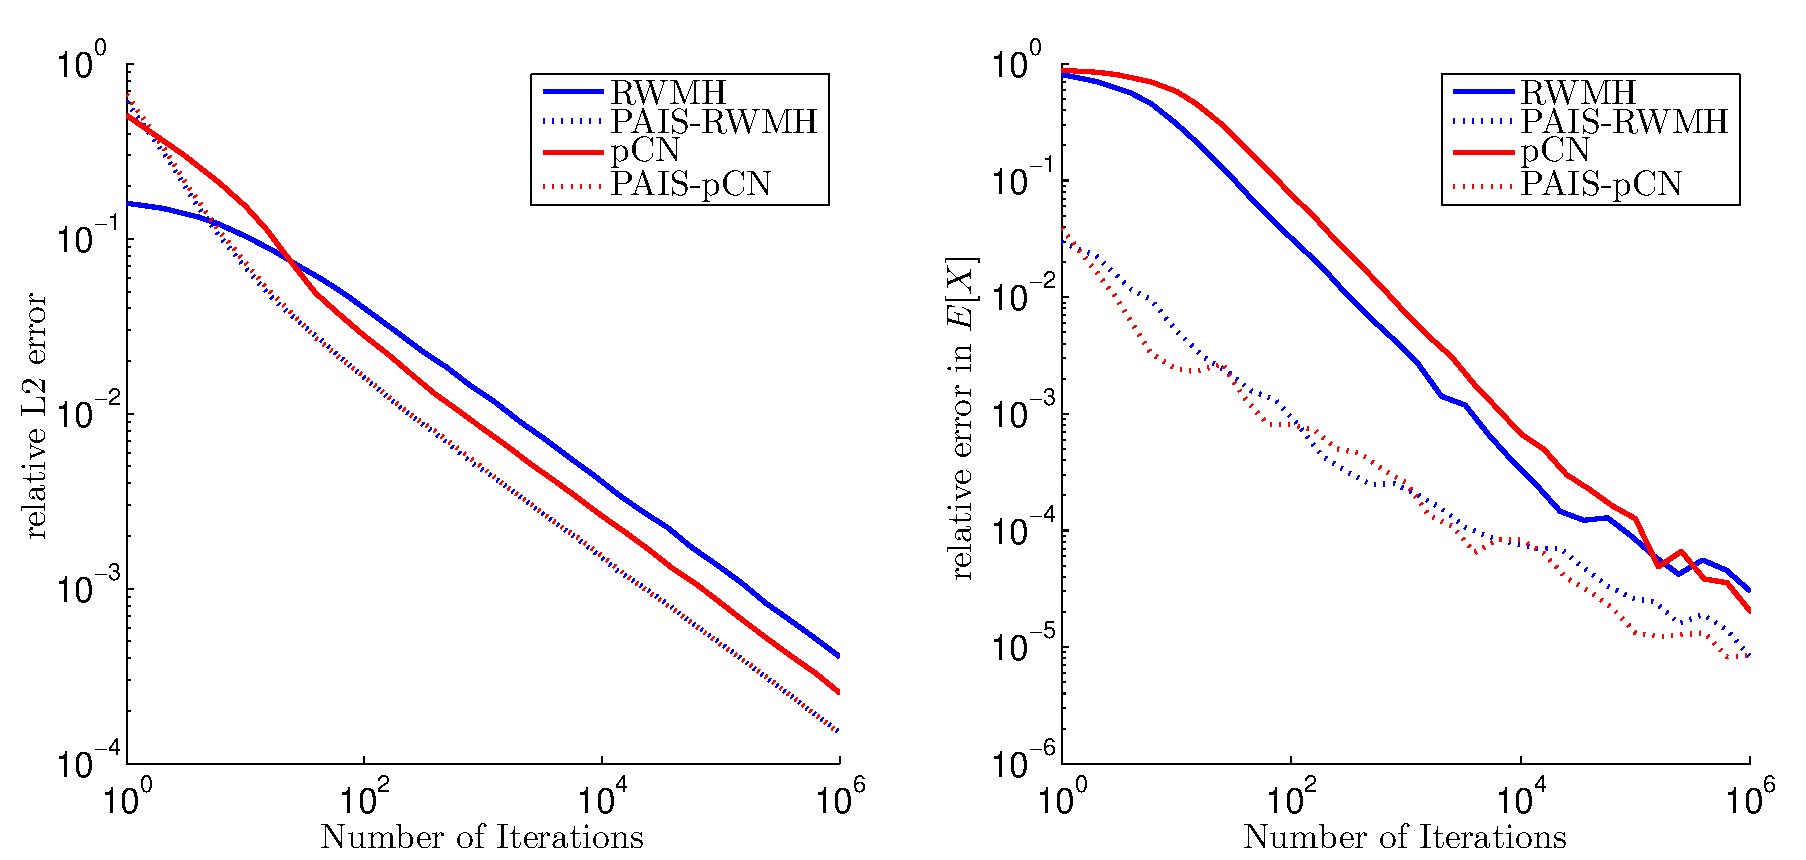
\includegraphics[width=\textwidth]{figures/RWMH1-pCN1}
\end{center}
\caption{RWMH vs pCN algorithms and with their PAIS variants.}
\label{fig:RWMH1}
\end{figure}
\begin{figure}[h]
\begin{center}
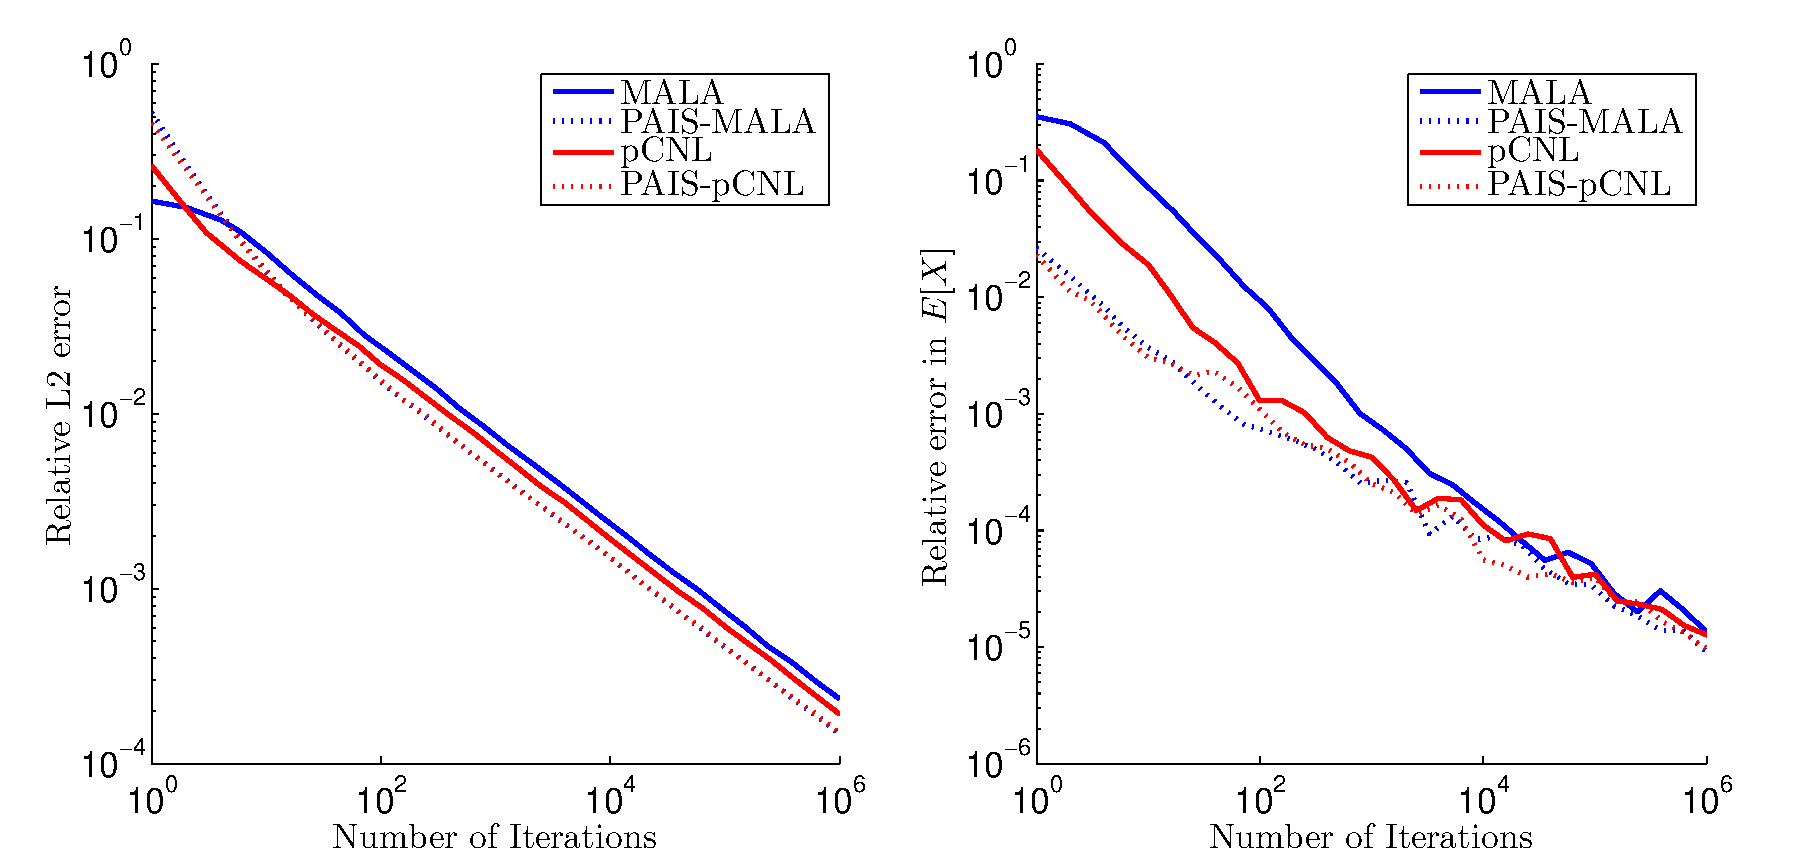
\includegraphics[width=\textwidth]{figures/MALA1-pCNL1}
\end{center}
\caption{MALA vs pCNL algorithms and with their PAIS variants.}
\label{fig:MALA1}
\end{figure}

\FloatBarrier\newpage
\section{Problem 2}
\[
	\mathcal{G}(u) = u, \quad \mu_0 \sim \mathcal{N}(0, 0.01), \quad \mu_\varepsilon \sim \mathcal{N}(0, 0.01), \quad D = 3.9980.
\]
\begin{figure}[h]
\begin{center}
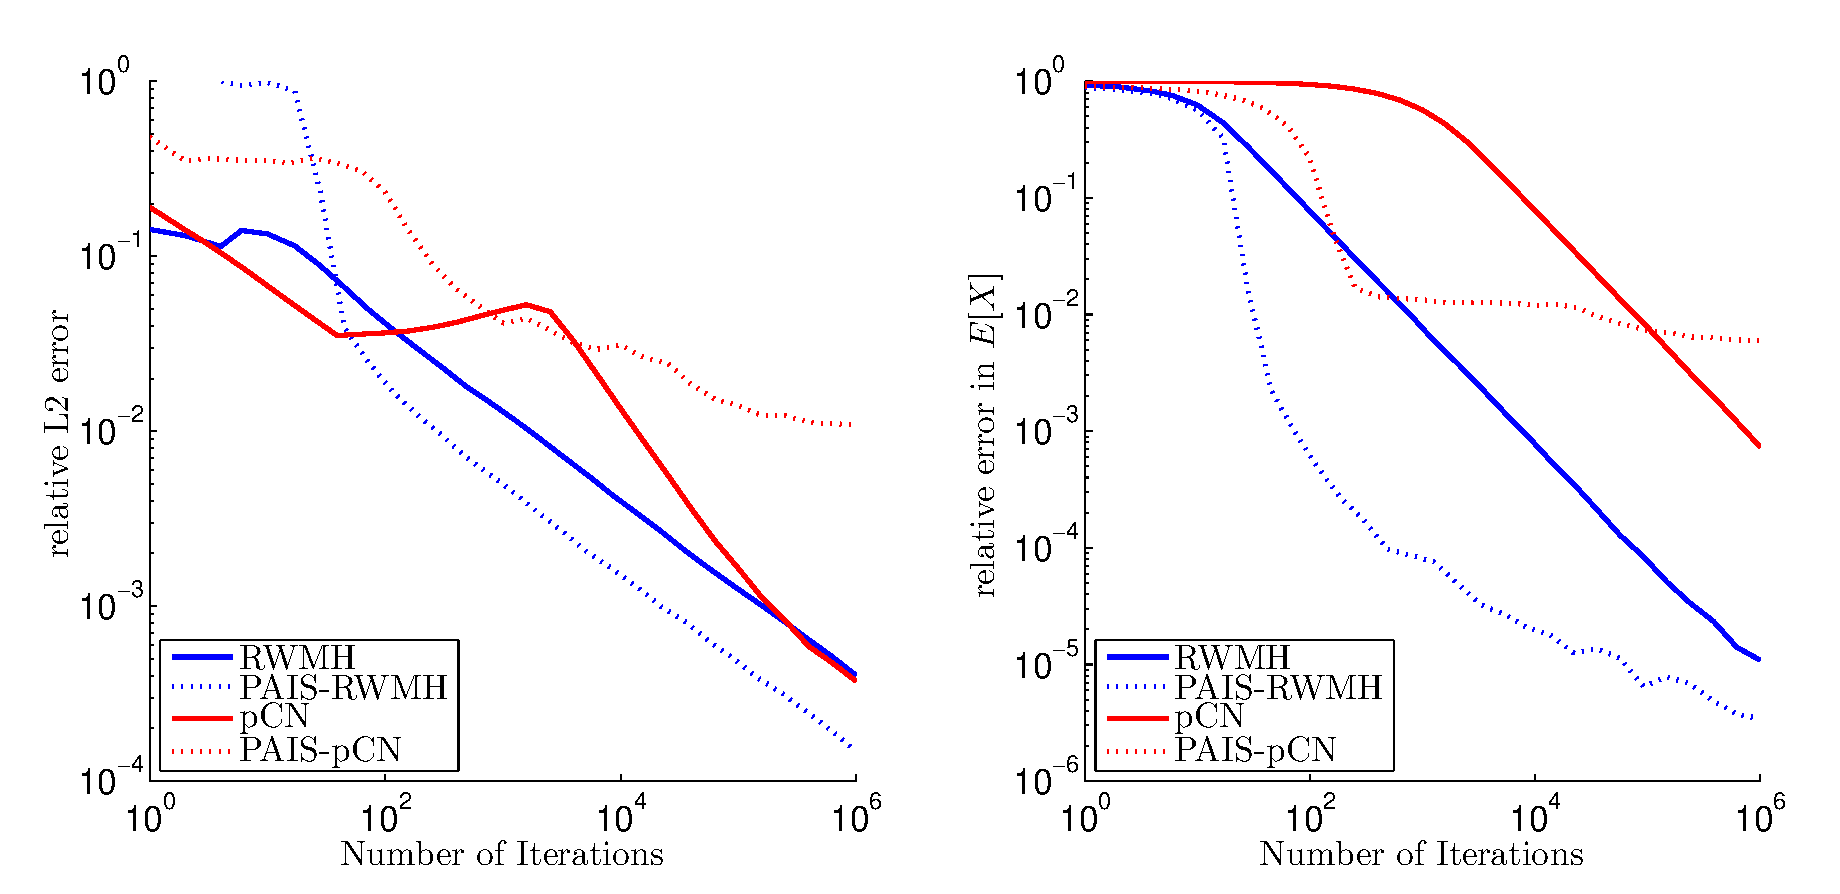
\includegraphics[width=\textwidth]{figures/RWMH2-pCN2}
\end{center}
\caption{RWMH vs pCN algorithms and with their PAIS variants.}
\label{fig:RWMH1}
\end{figure}
\begin{figure}[h]
\begin{center}
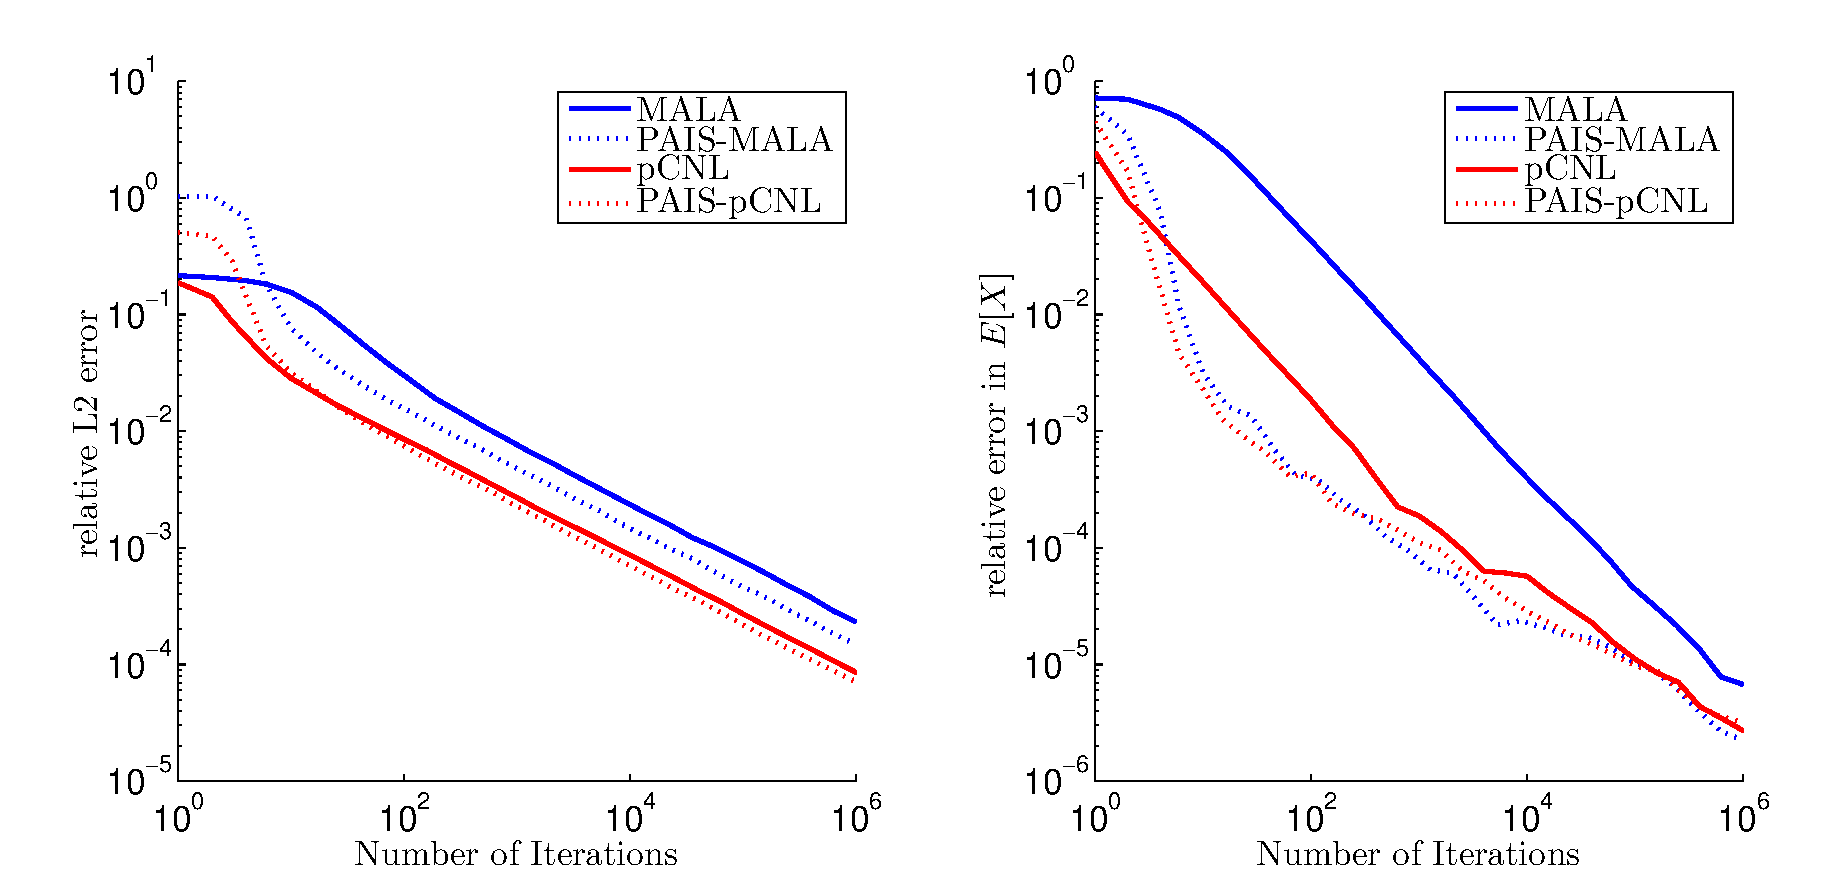
\includegraphics[width=\textwidth]{figures/MALA2-pCNL2}
\end{center}
\caption{MALA vs pCNL algorithms and with their PAIS variants.}
\label{fig:MALA1}
\end{figure}

\FloatBarrier\newpage
\section{Problem 3}
\[
	\mathcal{G}(u) = u^2, \quad \mu_0 \sim \mathcal{N}(0, 0.25), \quad \mu_\varepsilon \sim \mathcal{N}(0, 0.1), \quad D = 0.9213.
\]
\begin{figure}[h]
\begin{center}
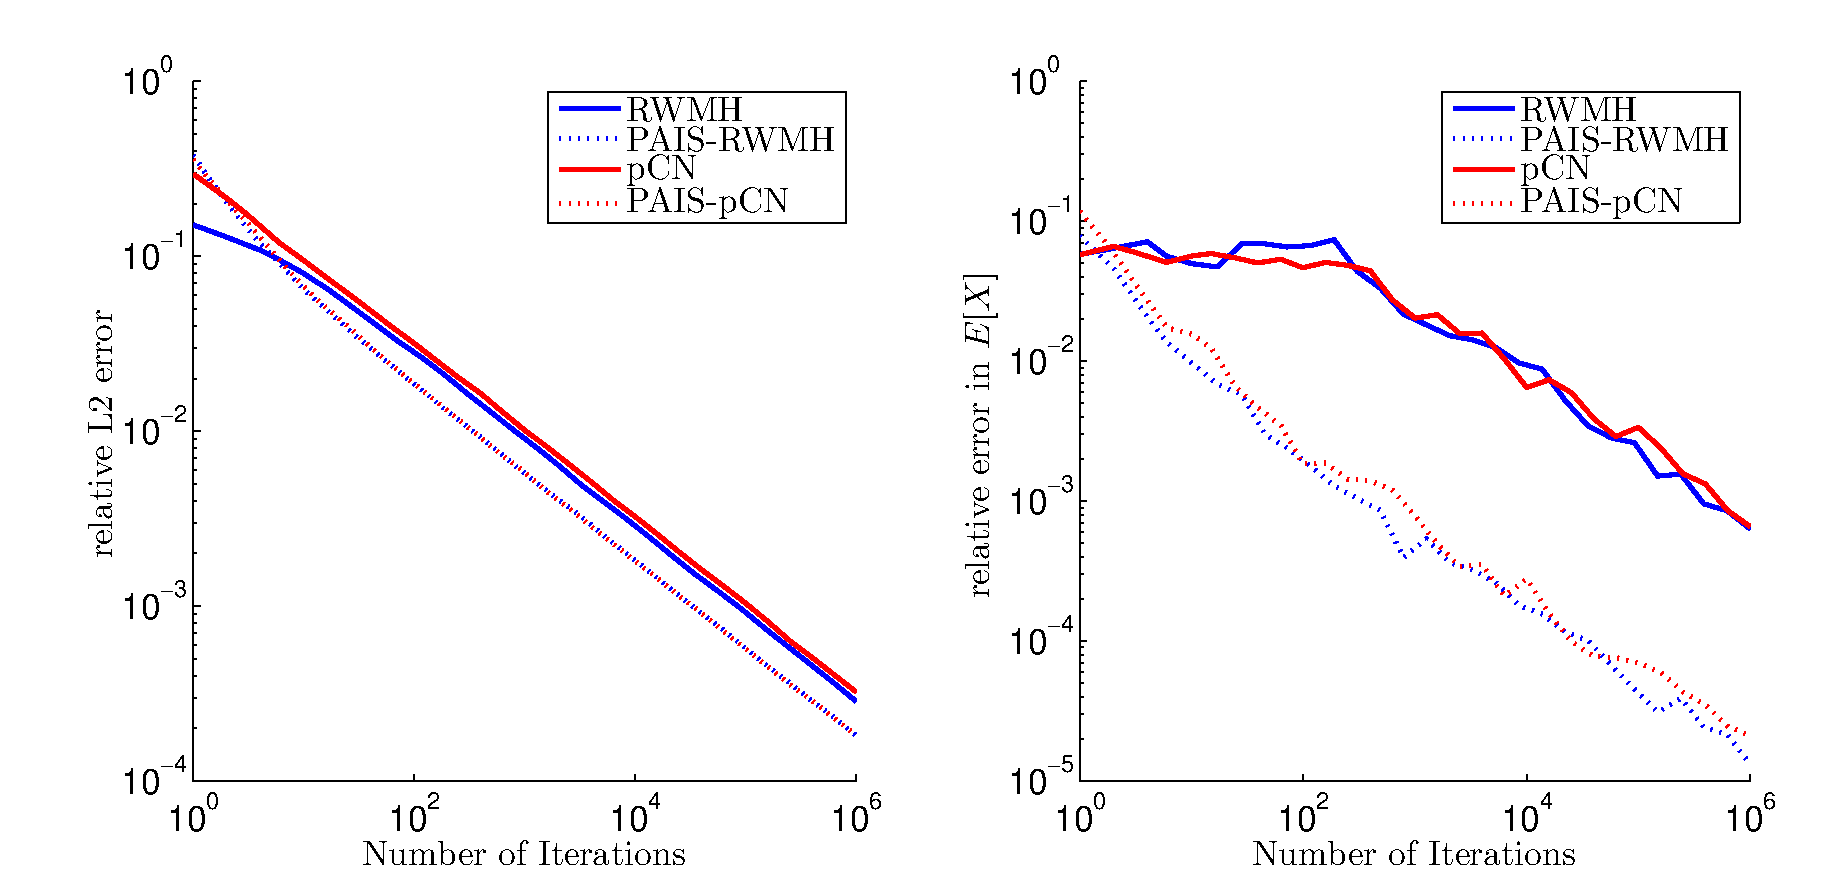
\includegraphics[width=\textwidth]{figures/RWMH3-pCN3}
\end{center}
\caption{RWMH vs pCN algorithms and with their PAIS variants.}
\label{fig:RWMH1}
\end{figure}
\begin{figure}[h]
\begin{center}
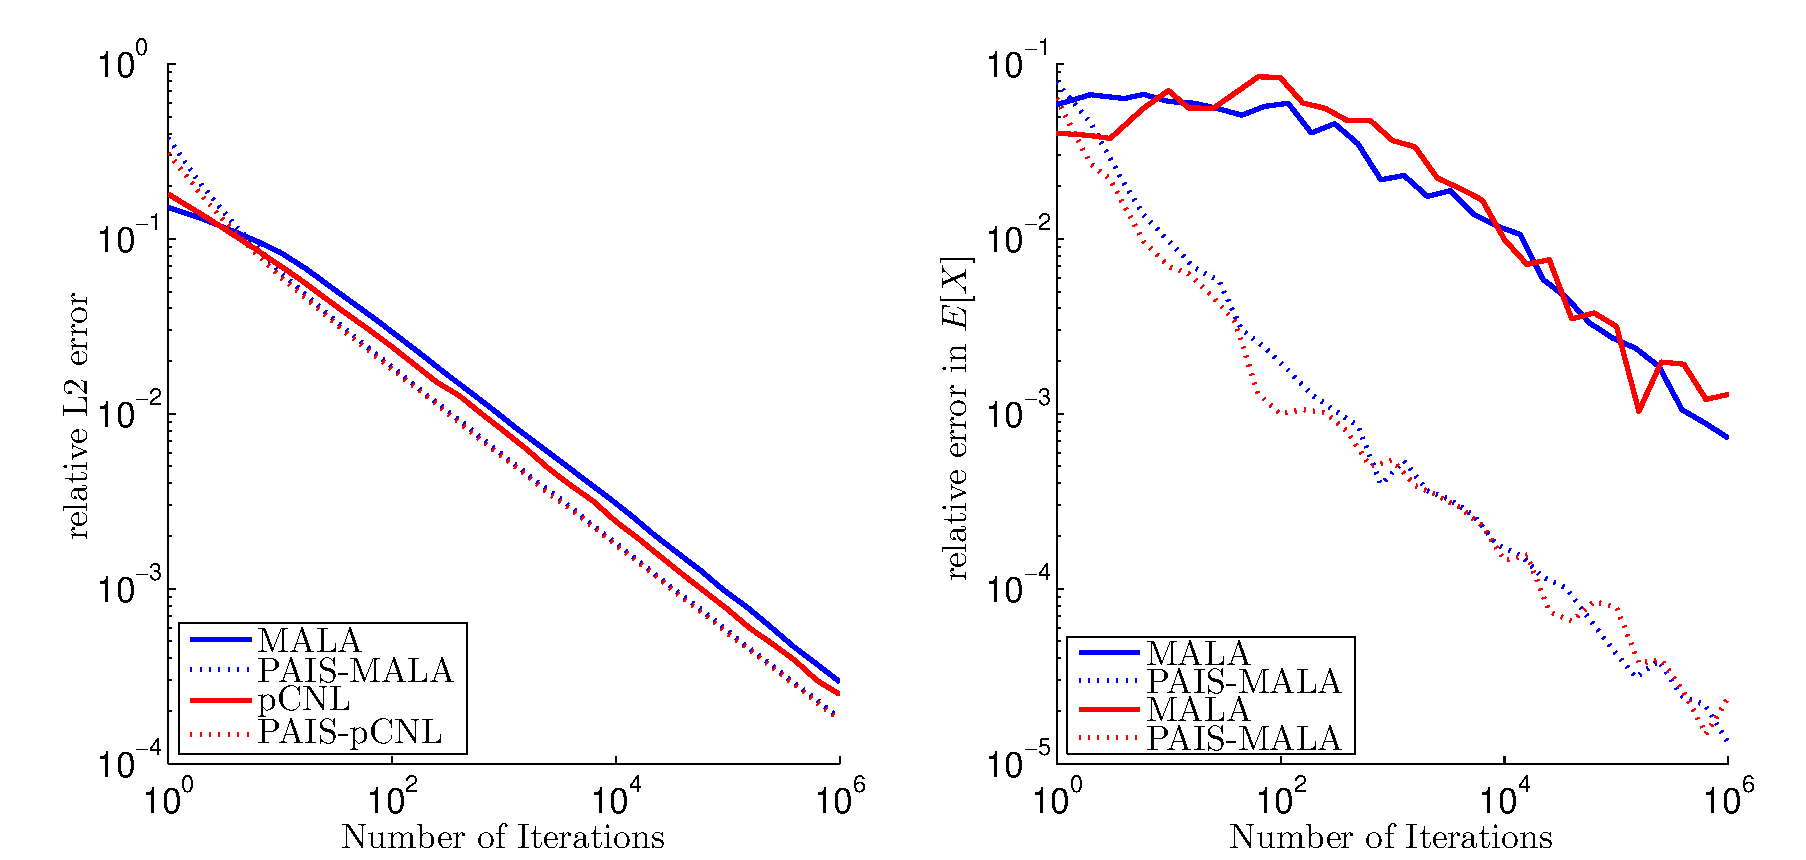
\includegraphics[width=\textwidth]{figures/MALA3-pCNL3}
\end{center}
\caption{MALA vs pCNL algorithms and with their PAIS variants.}
\label{fig:MALA1}
\end{figure}

\FloatBarrier\newpage
\section{Problem 4}
\[
	\mathcal{G}(u) = u^2, \quad \mu_0 \sim \mathcal{N}(0, 0.25), \quad \mu_\varepsilon \sim \mathcal{N}(0, 0.1), \quad D = 1.9487.
\]
\begin{figure}[h]
\begin{center}
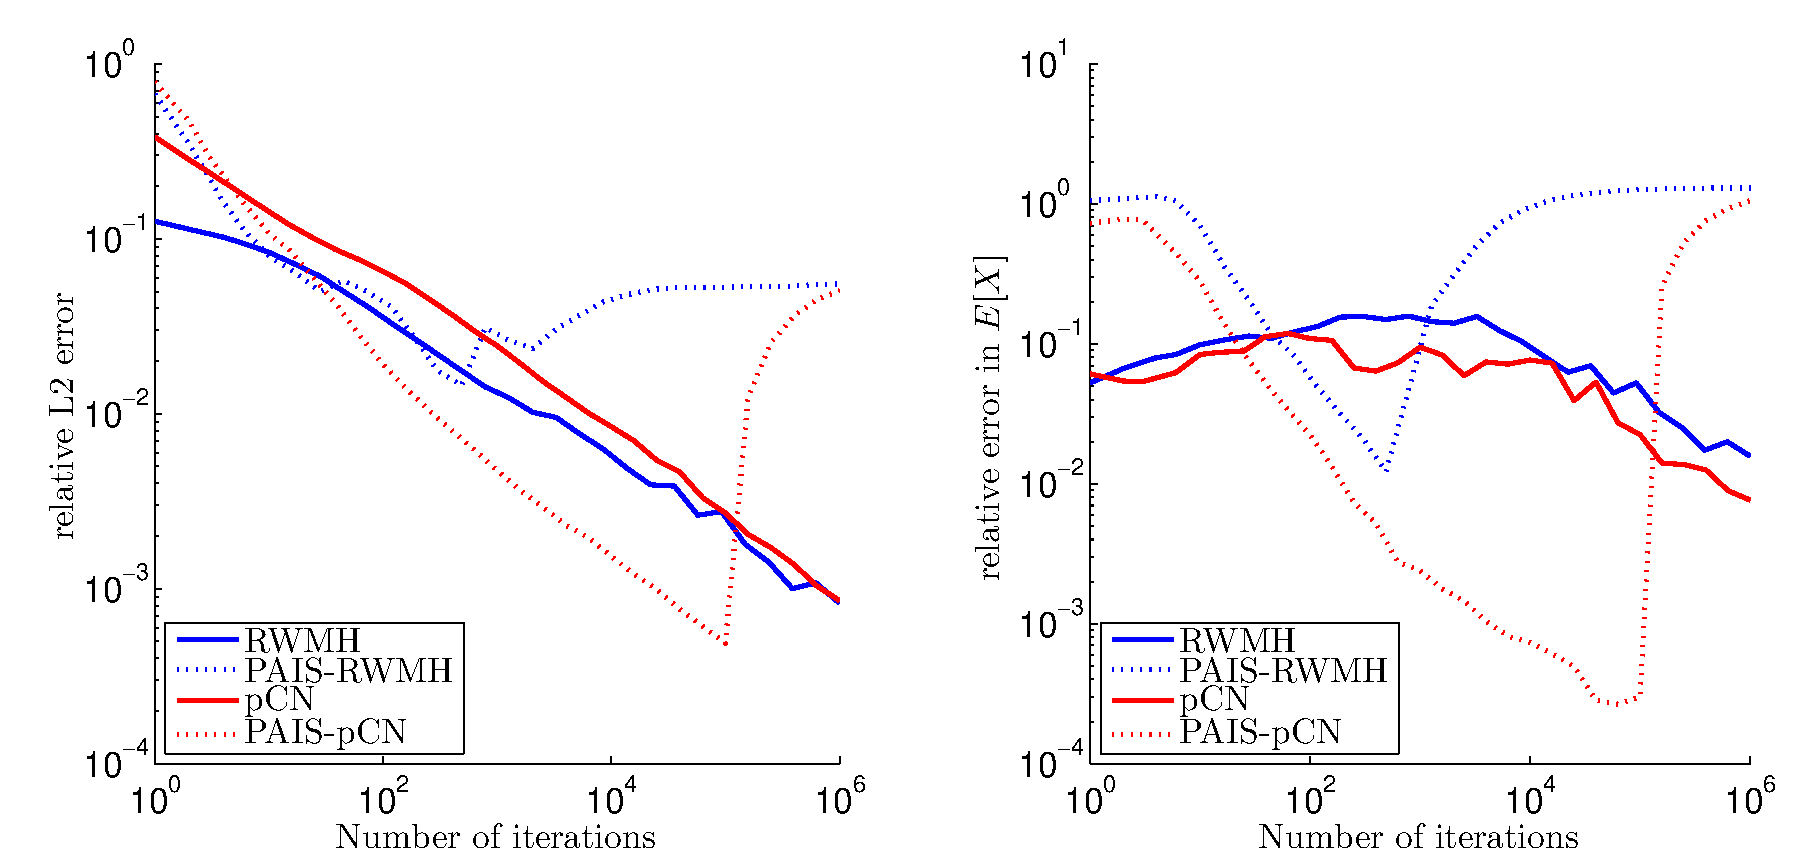
\includegraphics[width=\textwidth]{figures/RWMH4-pCN4}
\end{center}
\caption{RWMH vs pCN algorithms and with their PAIS variants.}
\label{fig:RWMH1}
\end{figure}
\begin{figure}[h]
\begin{center}
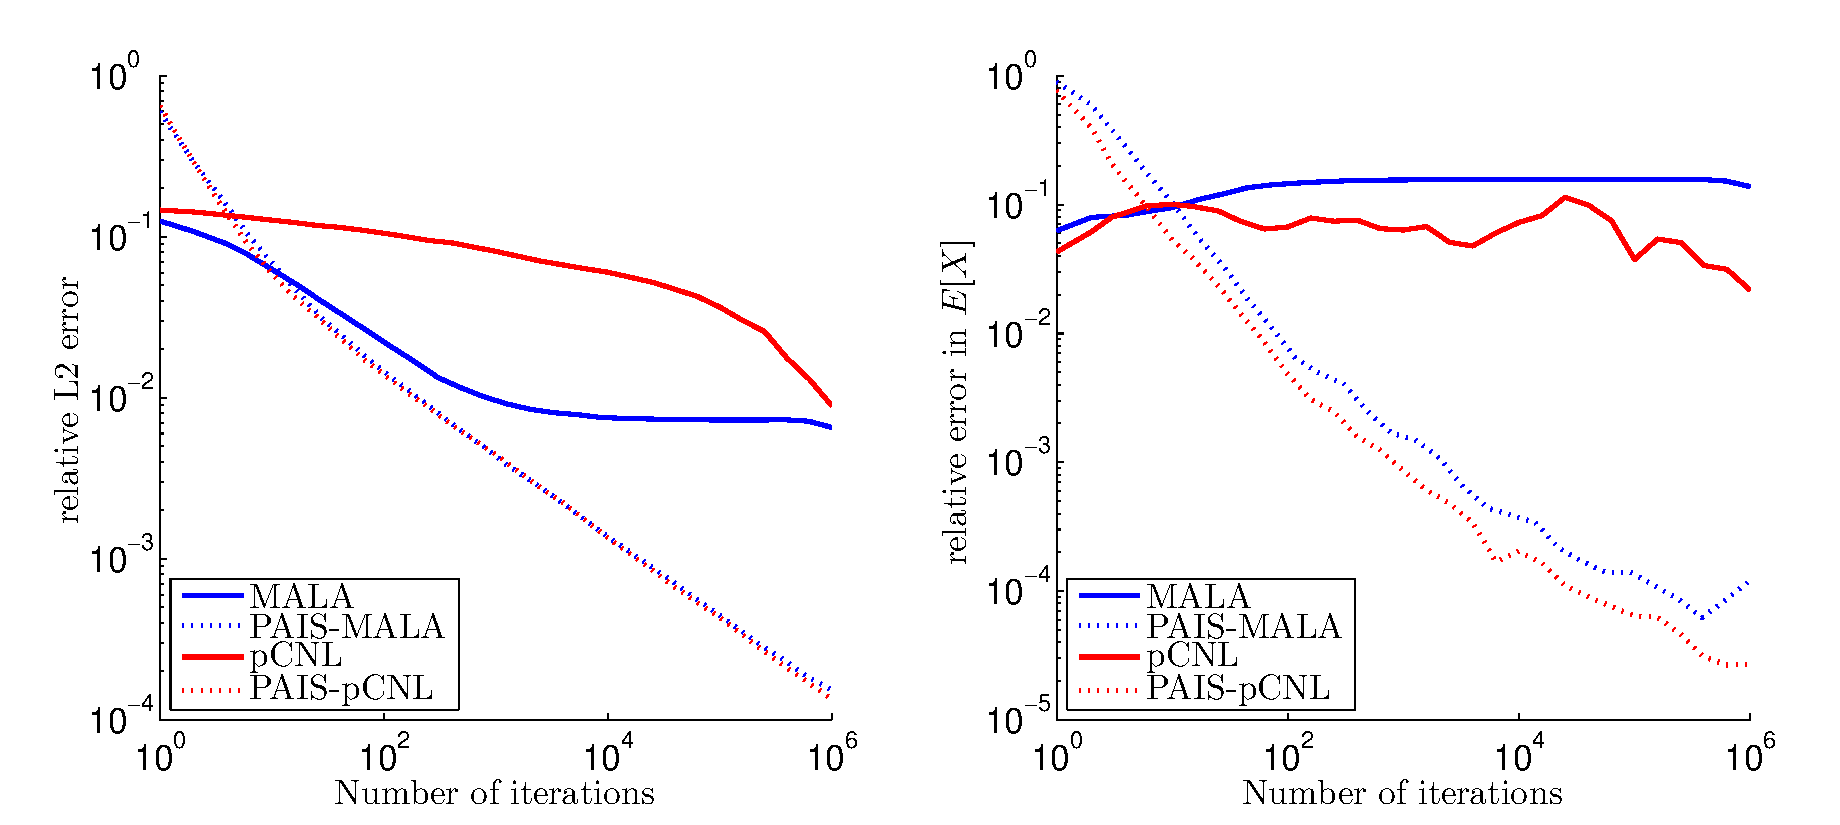
\includegraphics[width=\textwidth]{figures/MALA4-pCNL4}
\end{center}
\caption{MALA vs pCNL algorithms and with their PAIS variants.}
\label{fig:MALA1}
\end{figure}

\end{document}
